
模块允许程序员为代码定义API。代码可能由多个类、多个文件、几个函数和包括模板在内的各种辅助实用程序组成。通过使用关键字export,可以指定导出的内容为模块的API,该模块包装提供特定功能的所有代码。因此,可以为在不同文件中实现的组件定义一个干净的API。

让我们看几个简单的例子,它们在一个文件中声明一个模块,然后在另一个文件中使用这个模块。

\mySubsubsection{16.1.1}{实现和导出模块}

模块的API规范定义在其主接口(正式名称为主模块接口单元)中,每个模块只有一次:

\filename{modules/mod0.cppm}

\begin{cpp}
export module Square; // declare module Square

int square(int i);

export class Square {
private:
	int value;
public:
	Square(int i)
	: value{square(i)} {
	}
	int getValue() const {
		return value;
	}
};
	
export template<typename T>
Square toSquare(const T& x) {
	return Square{x};
}
	
int square(int i) {
	return i * i;
}
\end{cpp}

可能认识到的第一件事是,该文件使用了一个新的文件扩展名:.cppm。模块文件的扩展名还不清楚。稍后我们将讨论编译器对模块文件的处理。

主接口的关键是使用名称Square声明和导出模块的那行:

\begin{cpp}
export module Square; // declare module Square
\end{cpp}

请注意,该名称仅用作导入模块的标识符,不会引入新的作用域或命名空间。模块导出的任何名称仍然在导出时所在的作用域中。

模块的名称可以包含句点,而句点在C++中使用的任何其他类型的标识符中都是无效的,作为模块名称标识符的字符句点是有效的,并且没有特殊含义。例如:

\begin{cpp}
export module Math.Square; // declare module “Math.Square”
\end{cpp}

除了使用句点具有视觉效果外,这除了用“MathDotSquare”命名模块之外没有其他效果。period可以用来表示由组件或项目建立的模块之间的一些逻辑关系。使用它们不会产生句法或形式上的后果。

模块的公共API由使用关键字export显式导出的所有内容定义。本例中,我们导出了类Square和函数模板toSquare<>():

\begin{cpp}
export class Square {
	...
};

export template<typename T>
Square toSquare(const T& x) {
	...
}
\end{cpp}

其他所有内容都不能导出,也不能被导入模块的代码直接使用(将在后面讨论如何可以访问未导出的模块符号,但不可见)。因此,没有导出的函数square()不能被导入该模块的代码使用。

该文件看起来像一个头文件,但有以下区别:

\begin{itemize}
\item 
有模块声明的那一行。

\item 
符号、类型、函数(甚至模板)可以通过export导出。

\item 
不需要内联来定义函数。

\item 
不需要宏定义保护。
\end{itemize}

然而,模块文件不仅仅是一个改进的头文件。模块文件可以同时扮演头文件和源文件的角色,可以包含声明和定义。此外,在模块文件中,不必使用内联或预处理器保护来指定定义。当模块导出的实体被不同的翻译单元导入时,不能违反同一定义规则。

每个模块必须有一个指定名称的主接口文件,模块的名称与模块内的任何符号都不冲突,也没有隐式地引入命名空间。因此,模块可以具有其(主要)命名空间、类或函数的名称。在实践中,模块名可能经常与导出符号的命名空间相匹配,但需要这是显式实现。

\mySubsubsection{16.1.2}{编译模块单元}

模块文件可以同时具有声明和定义,所以可以看作是头文件和源文件的组合。可用它做两件事:

\begin{itemize}
\item 
\textbf{预编译声明} (包括所有泛型代码),将声明转换为特定于编译器的格式

\item 
\textbf{定义编译方式},创建通常的目标文件
\end{itemize}

\begin{center}
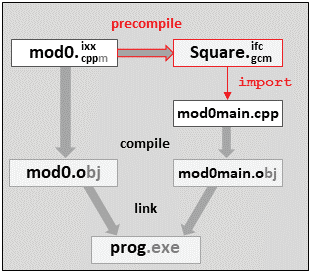
\includegraphics[width=0.6\textwidth]{content/chapter16/images/1.png}\\
图16.1 处理C++的模块
\end{center}

假设有主模块接口mod0,必须用两种方式处理它,如图16.1所示:

\begin{itemize}
\item 
必须预编译mod0.cppm,创建一个包含所有导出声明(包括预编译的模板定义)的预编译模块文件,由模块Square的名称标识,而不是源文件的名称。

\item
必须编译mod0.cppm,创建一个对象文件mod0.o或mod0.obj与汇编代码的所有定义,可以直接编译。
\end{itemize}

如前所述,源模块文件不需要特定的文件扩展名,在这里使用.cppm。预编译模块文件也没有标准化后缀,这是由编译器决定的。默认情况下,有以下情况:

\begin{itemize}
\item 
gcc/g++对预编译文件使用.gcm(并将它们放在gcm.cache子目录中)。

\item
Visual C++对预编译文件使用.ifc(并将它们放在本地目录中)。
\end{itemize}

我们将在后面详细讨论用于处理模块单元的文件后缀和选项。

请注意,要成功编译导入模块的源文件,需要模块的预编译工件可用。因此,必须在预编译mod0.cppm前编译mod0test.cpp。若没有遵循正确的顺序,可能会导入指定模块的非最新版本此,所以不允许循环导入依赖关系。

与其他编程语言相比,C++不要求模块具有特殊的文件名或位于特殊目录中。任何C++文件都可以定义一个模块(但只有一个),模块的名称不必与文件的名称或位置有任何关系。

当然,以某种方式保持文件名和模块名同步是很有意义的,但这个决定最终取决于开发者的偏好,以及对所使用的配置管理和构建系统。

\mySubsubsection{16.1.3}{导入和使用模块}

要在程序中使用模块的代码,必须以其名称导入该模块。下面是一个简单的程序示例,仅使用上面定义的模块Square:

\filename{modules/mod0main.cpp}

\begin{cpp}
#include <iostream>

import Square; // import module “Square”

int main()
{
	Square x = toSquare(42);
	std::cout << x.getValue() << '\n';
}
\end{cpp}

有

\begin{cpp}
import Square; // import module “Square”
\end{cpp}

从模块Square中导入所有导出的符号,则可以使用导出的类Square和函数模板toSquare<>()。

使用未导出的模块中的任何符号都会导致编译时错误:

\begin{cpp}
import Square; // import module ”Square”

square(42) // ERROR: square() not exported
\end{cpp}

再次注意,模块不会自动引入新的命名空间,在导出模块时所处的作用域中使用导出的模块符号。若希望将模块中的所有内容导出到其自己的命名空间中,则可以导出整个命名空间。

\mySubsubsection{16.1.4}{可及与可见}

使用模块时,一个新的区别就出现了:可达性与可见性。在导出数据时,可能无法看到并直接使用模块的名称或符号,虽然可以间接地使用。

当导出的API提供对未导出的类型的访问时,可能会出现可访问但不可见的符号。考虑下面的例子:

\begin{cpp}
export module ModReach; // declare module ModReach

struct Data { // declare a type not exported
	int value;
};

export struct Customer { // declare an exported type
private:
	Data data;
public:
	Customer(int i)
	: data{i} {
	}
	Data getData() const { // yield a type not exported
		return data;
	}
};
\end{cpp}

导入该模块时,Data类型不可见,因此不能直接使用:

\begin{cpp}
import ModReach;
...

Data d{11}; // ERROR: type Data not exported
Customer c{42};
const Data& dr = c.getData(); // ERROR: type Data not exported
\end{cpp}

但类型Data是可访问的,因此可以间接使用:

\begin{cpp}
import ModReach;
...

Customer c{42};
const auto& dr = c.getData(); // OK: type Data is used
auto d = c.getData(); // OK: d has type Data
std::cout << d.value << '\n'; // OK: type Data is used
\end{cpp}

甚至可以像下面这样声明一个Data类型的对象:

\begin{cpp}
decltype(std::declval<Customer>().getData()) d; // d has non-exported type Data
\end{cpp}

通过使用std::declval<>(),对假定的Customer类型对象调用getData()。因此,若为Customer类型的对象调用getData(),则使用Data类型声明它的返回类型。

私有模块片段可以用来限制间接导出的类和函数的可达性。

稍后将详细讨论导出符号的可见性和可达性。

\mySubsubsection{16.1.5}{模块和命名空间}

如前所述,模块的符号导入到与导出时相同的作用域中。与其他一些编程语言不同,C++模块不会自动为模块引入命名空间。

因此,可以将模块中的所有内容,导出到具有其命名空间中。可以通过两种方式做到这:

\begin{itemize}
\item 
在命名空间中使用export指定要导出的组件:
 
\begin{cpp}
export module Square; // declare module ”Square”

namespace Square {
	int square(int i);
	
	export class Square {
		...
	};
	
	export template<typename T>
	Square toSquare(const T& x) {
		...
	}
	
	int square(int i) { // not exported
		...
	}
}
\end{cpp}

\item 
在export声明的命名空间中指定想要导出的内容:

\begin{cpp}
export module Square; // declare module ”Square”

int square(int i);

export namespace Square {
	class Square {
		...
	};
	
	template<typename T>
	Square toSquare(const T& x) {
		...
	}
}

int square(int i) { // not exported
	...
}
\end{cpp}

\end{itemize}

这两种情况下,模块都会导出类Square::Square和Square::toSquare<>()(因此,即使没有使用export标记,符号的命名空间也会导出)。

现在使用该模块的方式如下所示:

\begin{cpp}
#include <iostream>

import Square; // import module ”Square”

int main()
{
	Square::Square x = Square::toSquare(42);
	std::cout << v.getValue() << '\n';
}
\end{cpp}

